\chapter{Results}\label{CH:results}

We analyze the Torchbearer system on two fronts: first, we examine the differences between pipelines on a performance and efficiency level, comparing execution cost, execution time and similarity between results. Second, we perform a field study with real drivers using the Torchbearer system to navigate an unknown route, comparing cognitive load, driving performance and perceived task difficulty between all four pipelines and a control. Our aim with these analyses is to understand the effectiveness of human versus machine methodologies for landmark selection and to determine the efficacy of the overall system for improving drivers' cognitive load and performance during naivgation.

\section{Pipeline Comparison}

To evaluate the differences in efficiency, cost and solution overlap we created a test set of 400 maneuver points in San Francisco, California, using an existing dataset \cite{sfIntersections} of geographic coordinates for all intersections in the city. Maneuver points were created at random by selecting an intersection and a route leading into it; the bearing for maneuver point was computed by measuring the angle between the two points closest to the intersection in a poly line representation of the route (see \ref{fig:polyline}).

\begin{figure}[htbp]
  \centering
  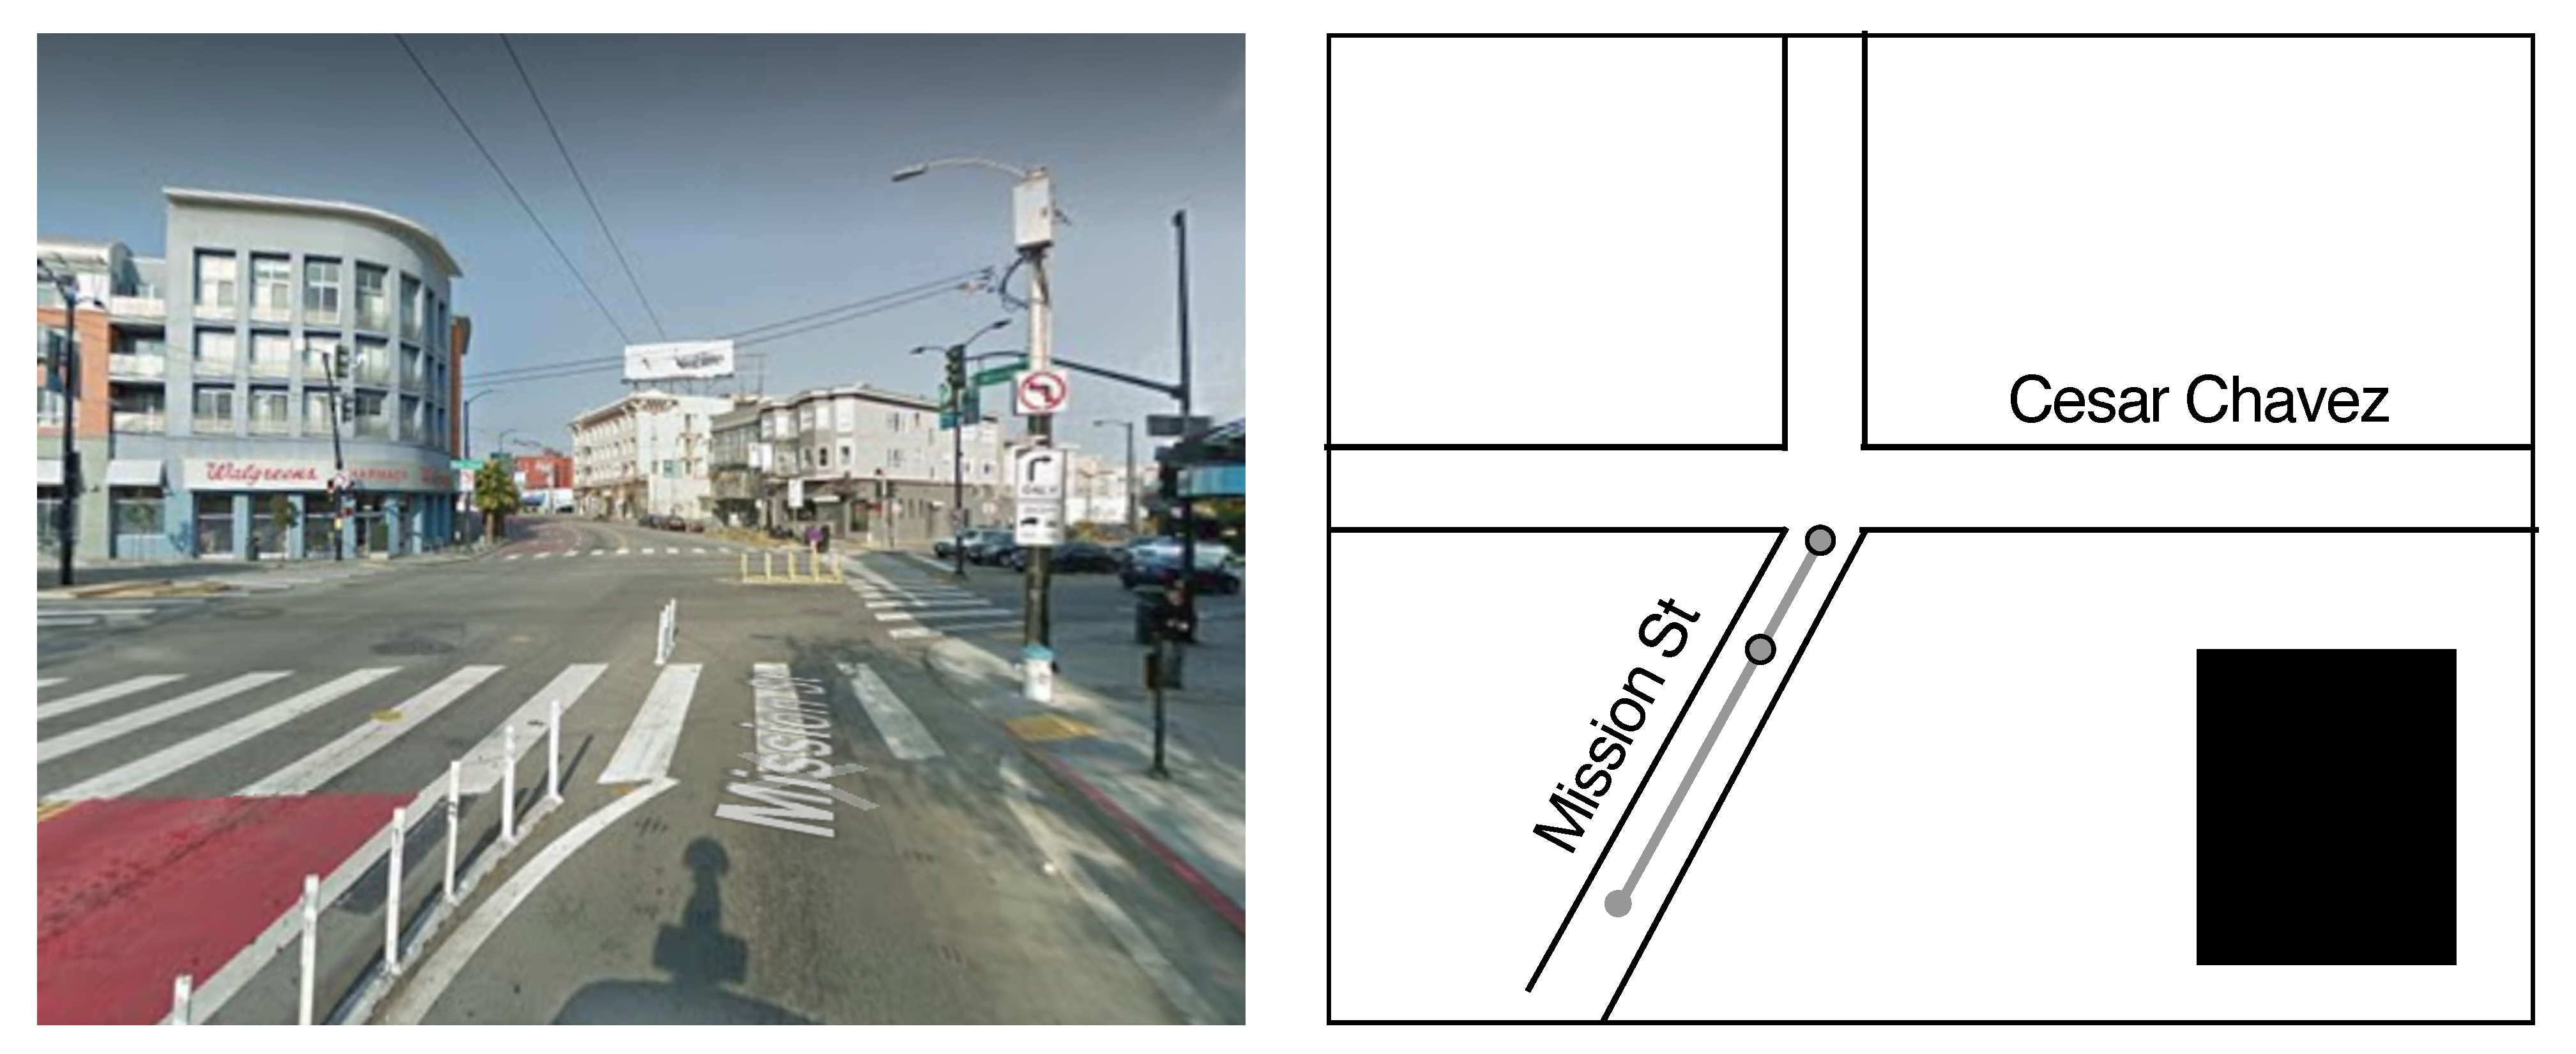
\includegraphics[width=0.6\textwidth]{images/POLYLINE.pdf}
  \caption{A hypothetical intersection in the SF test set. The grey line is a polyline representative of the selected route leading into the intersection. To find the bearing for the bearing value for the Torchbearer maneuver point we calculate the angle w.r.t. due north between the two points outlined in black.}
  \label{fig:polyline}
\end{figure}

Each maneuver point was processed through each of the four Torchbearer pipelines, resulting in a balanced result set of 1,600 pipeline executions.

\subsection{A Comparison of Pipeline Cost}

Torchbearer pipelines incur monetary cost when they use MTurk to gather human input. In an effort to compare the drawbacks and benefits of each pipeline, it is important to have an understanding of the differences in expenditure.

The cost incurred for the processing of each maneuver point is recorded in the Torchbearer database as the pipeline executes; anytime a HIT is submitted to MTurk the cost is increased by $nc$ where $n$ is the number of workers who will complete the HIT and $c$ is the amount to be paid to each worker. For this experiment we paid workers \$0.0.5 for a saliency selection HIT, \$0.05 for a landmark description HIT and \$0.03 for a landmark verification HIT. These amounts were selected based on observational analysis of Mechanical Turk pricing for similar object-detection-related tasks; we aimed to offer above average pay for each type of HIT to avoid low pay as a confounding variable in work quality. The marginal pipeline costs (the cost of processing an additional maneuver point) are shown in \ref{fig:plot:cost}

\begin{figure}[htbp]
  \centering
  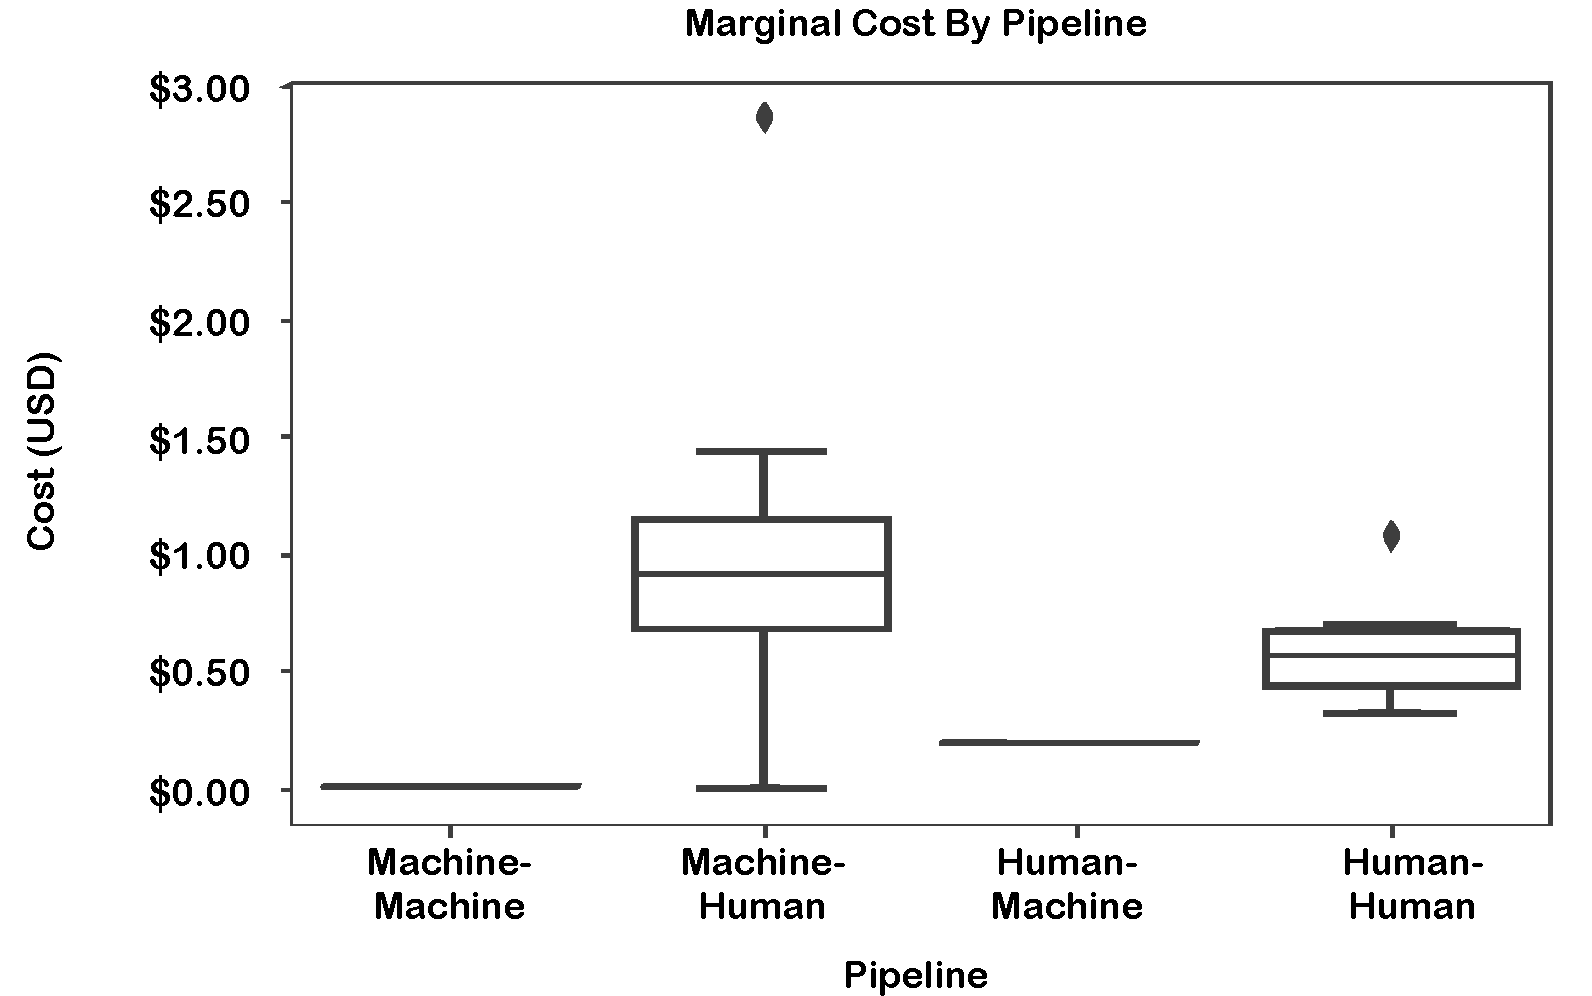
\includegraphics[width=0.6\textwidth]{images/plot_cost.pdf}
  \label{fig:plot:cost}
\end{figure}

The marginal cost of the Machine-Machine pipeline is \$0.00, with no variance, since of course this pipeline makes no requests of human workers. The results for the Human-Machine pipeline are similarly simplistic---this pipeline makes 


indicative of contention